%\newpage
  \begin{titlepage}
    \vspace*{\fill}
      \part{Introduction}
    \vspace*{\fill}
  \end{titlepage}

\startcontents[parts]

\phantomsection
\chapter*{Contents}

\textit{The main motive of this project is to understand facial expression recognition systems and their applications. A review of the architecture of such systems will be done, along with a state of the art of already existing algorithms. After this study, issues coming along with this kind of recognition system will be studied. In the last part, the requirements of this project will be formulated.}

\vspace{\baselineskip}

\printcontents[parts]{}{-1}{\setcounter{tocdepth}{1}}

\pagebreak

\phantomsection
\chapter{Motivations}

\noindent A facial expression is a visible manifestation of the effective state, cognitive activity, intent, personality, and psychopathology of a person \cite{DON99}; facial expressions play a significant role in human dialogue and interaction. Indeed, facial expressions carry more informations than mere speech, informations on which humans can relay for interaction. Facial expressions have a considerable effect on a listening interlocutor; a speaker facial expressions accounts for about 55 percent of the effect, 38 percent of the latter is conveyed by voice intonation and 7 percent by the spoken words \cite{PAN00}.
\newline

\noindent Since Antiquity, researchers have been interested in emotion and more particularly in emotion recognition. But one of the important studies on facial expression analysis impacting on the modern day science of automatic facial expression recognition was the work carried out by Charles Darwin \cite{BET12}. In 1872, Darwin wrote a treatise that established general expression principles and expression means for both humans and animals \cite{DAR04}. He also classified various kinds of expressions. This can be considered as the beginning of facial expression recognition.
\newline

\noindent Now, with the emergence of new technologies and computers, research is now focused on computer-based automatic facial expression recognition. Because facial expressions are major factors in human interaction, this research field will broaden the domain of Human-Machine Interaction. Indeed, emotion recognition will enable computers to be more responsive to users' emotions, and allow interactions to become more and more realistic. 
\newline

\noindent Another domain where facial expression recognition is an important issue is robotics. With the advances made in robotics, robots nowadays tend to mimic human emotion and react as as human-like as possible, especially for humanoid robots. However, since robots are being more and more present in our daily lives, they need to understand and recognize human emotions.
\newline

\noindent A lot of real time applications in the robotics field have already been created. For example, Bartlett et al. have successfully used their face expression recognition system to develop an animated character that mirrors the expressions of the user (called CU Animate) \cite{BAR03}. They have also been successful in deploying the recognition system on Sony's Aibo Robot and ATR's RoboVie \cite{BAR03}. Another interesting application has been demonstrated by Anderson and McOwen, called "EmotiChat" \cite{AND06}. It is a regular chatroom, except the fact that their facial expression recognition system is connected to the chat and convert the users' facial expressions into emoticons. Because facial expression recognition systems' robustness and reliability are constantly increasing, lots of innovative applications will appear.
\newline

\noindent There are also various other domains where emotion recognition can be used: Telecommunications, behavioural science, video games, animations, psychiatry, automobile safety, affect-sensitive music jukeboxes and televisions, educational software, etc \cite{BET12}.
\newline

\noindent Our project focuses on real-time facial expression recognition from a video stream. Indeed, facial expression recognition can be performed \textit{statically} on input images, or \textit{dynamically} on video sequences. Systems can also be \textit{obtrusive}, or \textit{non-obtrusive}, the former based on a device mounted on the user's head or body, therefore following each of his movements and perform facial expression recognition without much losses, while the latter can encounter difficulties if the user is not properly situated. However, non-obtrusive systems allow more natural user interactions. We chose our system to be non-obtrusive, and will detail further its setup in the next section.
\newline

\phantomsection
\section{Environment Setup}

\vspace{\baselineskip}
\noindent Our system will use the camera embedded into a Microsoft Kinect to record the user's video input, and we will consider a casual use of the camera, with the user sitting in front of the computer, the camera being next to it, as seen in \textbf{\color{red} Insert picture of the setting \& ref to figure}. This camera provides a 640$\times$480 pixels frame resolution, while recording at 30 FPS.
\newline

\noindent For development and training purposes we will use some pre-existing emotion datasets, in order to validate the efficiency of the system before testing it in real conditions.
\newline

\phantomsection
\section{Emotion Datasets}

\noindent Databases are very important for facial expression recognition system.
\newline

\noindent Using the same databases for studies that aims to improve existing systems is very useful. It allows to compare he results and to see if the new system is indeed better than the existing one. A lot of research studies work is based on the same databases than previous studies in order to compare the efficiency of their algorithm.
\newline

\noindent But databases are hard to construct. It has to fill all the requirements and that is why most of the work on facial expression recognition is based on existing databases. The hardest requirement to fill is to have a standardized database. Most of the actual databases use posed expressions and not spontaneous expression, and both are very different. New versions of the databases are coming out with spontaneous expressions in order to be more complete. Even with this transition from posed expressions to spontaneous expressions, there are other requirements that should be respected to have a database standardized for training and testing. It should contain images and video sequences and both should be of different resolutions. It should also contain people displaying expressions under different conditions: it could be change in the lighting, occlusions or rotations of the head \cite{BET12}.  
\newline

\noindent Following are the databases that will be used to test this facial expression recognition system. These are part of the databases that are popular, freely available and mostly used in the past few years.
\newline

\subsection{Japanese Female Facial Expression Database (JAFFE)}

\vspace{\baselineskip}
\noindent The database contains 213 images of 7 facial expressions (6 basic facial expressions: happy, angry, afraid, disgusted, sad, surprised + 1 neutral) posed by 10 Japanese female models. Each expression has been photographed three or four times. Each image has been rated on 6 emotion adjectives by 60 Japanese subjects. The database was planned and assembled by Miyuki Kamachi, Michael Lyons, and Jiro Gyoba \cite{JAFFE}.
\newline

\noindent This database contains only posed expressions. The photos have been taken under strict controlled conditions of similar lighting and with the hair tied away from the face \cite{BET12}. 
\newline

\noindent An example of images contained in the database is given by the figure~\ref{jaffe_7facialexpressions}. Here the subject is a woman and she displays 7 different emotional expressions (neutral, happy, angry, afraid, disgusted, sad, surprised): 
\newline

\begin{figure}[!h]
\begin{center}
\noindent 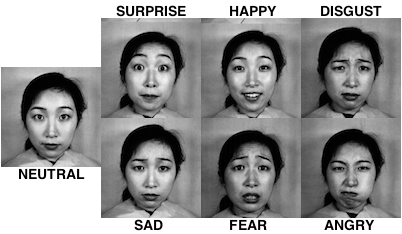
\includegraphics[scale=0.8]{figures/jaffe_7facialexpressions} 
\newline
\caption{example of images from JAFFE database}
\label{jaffe_7facialexpressions}
\end{center} 
\end{figure}

\subsection{Karolinska Directed Emotional Faces Database (KDEF)}

\vspace{\baselineskip}
\noindent The Karolinska Directed Emotional Faces (KDEF) is a set of totally 4900 pictures of human facial expressions of emotion. The material was developed in 1998 by Daniel Lundqvist, Anders Flykt and Professor Arne Ohman at Karolinska Institutet, Department of Clinical Neuroscience, Section of Psychology, Stockholm, Sweden \cite{KDEF}.
\newline

\noindent The material was originally developed to be used for psychological and medical research purposes. More specifically material was made to be particularly suitable for perception, attention, emotion, memory and backward masking experiments. Hence, particular attention was for instance paid to create a soft, even light, shooting expressions in multiple angles, use of uniform T-shirt colors, and use of a grid to center participants face during shooting, and positioning of eyes and mouths in fixed image coordinates during scanning \cite{KDEF}.
\newline

\noindent The set contains 70 individuals (35 males and 35 females), ranging from 20 to 30 years, each displaying 7 different emotional expressions (neutral, happy, angry, afraid, disgusted, sad, surprised),
each expression being photographed (twice) from 5 different angles (-90, -45, 0, +45, +90 degrees: i.e. full left profile, half left profile, straight, half right profile, full right profile)  \cite{KDEF}.
\newline

\noindent An example of images contained in the database is given by the figure~\ref{kdef_7facialexpressions}. Here the subject is a woman photographed from a straight angle and she displays 7 different emotional expressions (neutral, happy, angry, afraid, disgusted, sad, surprised): 
\newline

\begin{figure}[!h]
\begin{center}
\noindent 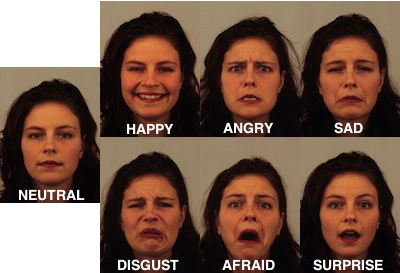
\includegraphics[scale=0.7]{figures/kdef_7facialexpressions} 
\newline
\caption{example of images from KDEF database}
\label{kdef_7facialexpressions}
\end{center} 
\end{figure}

\subsection{Montreal Set of Facial Displays of Emotion Database (MSFDE)}

\vspace{\baselineskip}
\noindent The database consists of emotional facial expressions by men and women of European, Asian, and African descent. Each expression was created using a directed facial action task and all expressions were FCAS coded to assure identical expressions across actors \cite{MSFDE}.
\newline

\noindent The set contains expressions of happiness, sadness, anger, fear, disgust, and embarrassment as well as a neutral expression for each actor. All expressions have been morphed into 5 different levels of intensity \cite{MSFDE}.
\newline

\noindent An example of images contained in the database is given in the figure~\ref{msfde_7facialexpressions}. Here the subject is an african woman and she displays 7 different emotional expressions (neutral, happy, angry, afraid, disgusted, sad, ashamed): 
\newline

\begin{figure}[!h]
\begin{center}
\noindent 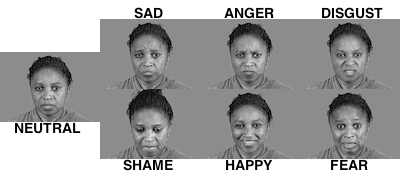
\includegraphics[scale=0.9]{figures/msfde_7facialexpressions} 
\newline
\caption{example of images from MSDFE database}
\label{msfde_7facialexpressions}
\end{center} 
\end{figure}







\newpage
\phantom\phantomsection
\chapter{Facial expression recognition}

\noindent After having stated the conditions and motivations of our project, we will now describe an overview of the system we will implement. A facial recognition system can roughly be summed up as classification applied to a pre-processed image. The image processing steps, especially the feature extraction part, along with commonly used classification algorithms, will be detailed further in this chapter. Next sections will be about issues raised facial expression recognition systems, and key requirements these systems have to meet in order to be considered acceptable.

\section{General structure}

\noindent Facial expression recognition is a system enabling an automatic recognition of emotions displayed by a human face. Facial expression recognition can be image or video-based; it can also be computed real-time. Most of the time, researchers try to recognize emotions out of images of human faces. This can also be achieved real-time on video streams : While the person displays his/her emotions, the facial expression recognition system analyses the video, and detect in real-time the displayed emotion.
\newline

\noindent In both cases, facial expression recognition process is structured as follows:
\newline

\noindent 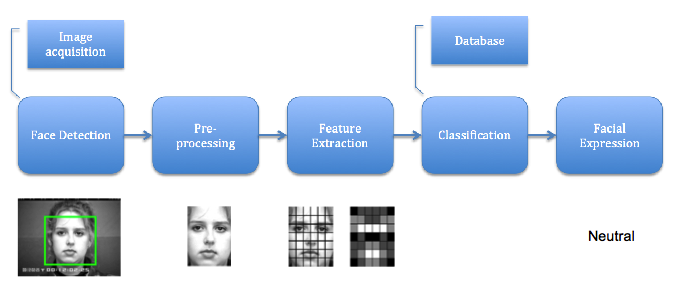
\includegraphics[scale=0.6]{figures/facial_expression_recognition_process}
\newline

\subsection{Image Acquisition}

\vspace{\baselineskip}
\noindent First step of the process is "Image Acquisition". Images used for facial expression recognition can be static images or image sequences. Image sequences give more informations about the facial expression, as the steps in muscles movement. About static images, facial expression recognition systems usually need 2D greyscale images as inputs. We can however expect future systems to use colour images; first because of the increasing affordability of technologies and devices capable of capturing images or image sequences; then because colours can give more information on emotions, i.e blushing \cite{CHI03}.
\newline

\subsection{Face Detection}

\vspace{\baselineskip}
\noindent Second step is "Face Detection". Indeed, in a static image and even more in an images sequence, this is an obvious need. Once the face has been detected, all other non-relevant information can be deleted, since only the face is needed. It could hence be included in the next step, which is "Pre-processing", but because of its importance it represents a step in itself. In a real-time facial expression recognition system working with image sequences, the face has to be detected, but also tracked. One of the most used and famous detection and tracking algorithm is the Viola-Jones Algorithm, which we will explain in detail later in this report. This algorithm can be trained to detect all kind of objects, but is mostly used for face detection. 
\newline

\subsection{Pre-processing}

\vspace{\baselineskip}
\noindent Third step is "Pre-processing", which is about applying image processing algorithms to the image, in order to prepare it for the next step. Pre-processing is usually about noise removal, normalization against the variation of pixel position or brightness, segmentation, location, or tracking of parts of the face. Emotion recognition is also sensitive to transformation, scaling and rotation of the head in the image or image sequence. In order to solve this problem, the image can be geometrically standardized. References used for this standardization are usually the eyes \cite{CHI03}.
\newline

\subsection{Features Extraction}

\vspace{\baselineskip}
\noindent Once the image has gone through the "Pre-processing" step, the next one is "Features Extraction". In this step, data is converted into a higher representation of shape, motion, colour, texture, and spatial configuration of the face or its components. One of the main goals of this step is to reduce the dimensionality of the input data. The reduction procedure should retain essential information possessing high discrimination power and high stability \cite{CHI03}. There are a lot of features extraction methods. The most famous are : Principal Component Analysis (PCA), Linear Discriminant Analysis (LDA), Problem Based Learning (PBL), Hidden Markov Models (HMM), Eigenfaces, Gabor Wavelets. The extracted data is then used in the "Classification" step.
\newline

\subsection{Classification}

\noindent The classification step marks the end of image processing steps (face detection, normalization, feature extraction). There are many kinds of classification algorithms, some of them can even be used in the feature extraction part, as stated in Section \ref{feat_x}. This step takes into input a model, previously trained with pre-processed data, and test data, which is feature vectors extracted from the image we want to label. Feature vectors from pre-processed data and train data have to be obtained using the same feature extraction algorithm. The chosen classifier then outputs a value corresponding to the label of the class the picture belongs to.

\phantomsection
\section{Feature extraction algorithms} \label{feat_x}

\vspace{\baselineskip}
\noindent Before developing a facial expression recognition project, it is important to know what already exists; the state of the art of facial expression recognition system. In this chapter, an overview will be given of the existing systems before to decide on a system for the project.
\newline

\noindent 2 main categories of feature extraction algorithms can be distinguished : \textit{appearance-based} or \textit{geometry-based}. The first ones are algorithms that try to find basic vectors characterising the whole picture, usually by a dimensionality reduction method. These algorithms lead to a simplification of the dataset, while retaining the main characteristics of the picture. However, these methods have to be carefully parametrized, so they do not encounter the "curse of dimensionality", which is about processing high-dimensional data.
\vspace{\baselineskip}

\noindent Examples of appearance-based methods : Principal Component Analysis, Linear Discriminant Analysis, Hidden Markov Models, Eigenfaces
\newline

\noindent The second type of feature extraction algorithms is geometry-based algorithms. These methods tend to locate important features, and build the feature vectors depending on those regions of interest. The key point of these methods is that the face is not a global structure anymore. Indeed, it has been summarized in a set of features regions, which are themselves translated into feature vectors.
\vspace{\baselineskip}

\noindent Examples of geometry-based methods : Gabor Wavelets, Local Binary Patterns
\newline

\subsection{Principal Component Analysis (PCA)}

\vspace{\baselineskip}
\noindent This is a statistical method; one of the most used in linear algebra. PCA is mainly used to reduce high dimensionality of data and to obtain the most important information from this data. Because Facial Expression Recognition needs to reduce the dimensionality of data during features extraction, PCA is commonly used. It helps transforming high dimensionality of data to a new coordinate system of lower dimensions while still preserving the most important information. PCA computes a covariance matrix and a set of values called the eigenvalues and eigenvectors from the original data \cite{GAN08}. Since it is a statistical method, it can also be used in the classification step.
\newline

\subsection{Linear Discriminant Analysis (LDA)}

\vspace{\baselineskip}
\noindent Linear Discriminant Analysis is also a statistical method, used to classify a set of objects into groups. It is done by observing a set of features that describe the objects. LDA as PCA are used to establish a linear relationship between the dimensions of the data. The main difference is that LDA uses the linear relationship to model the differences into classes of objects and PCA does not take any differences into account in the linear relationship. The idea is to perform a linear transformation on the data to obtain a lower dimensional set of features \cite{GAN08}. Like PCA, LDA is also a classification algorithm.
\newline

\subsection{Local Binary Patterns (LBP)}

\vspace{\baselineskip}
\noindent This is an appearance-based method. It can be used to describe texture and shape. LBP extracts some informations from the neighbourhood of a central pixel. It compares the intensity values of the neighbourhood pixels with the intensity value of the central pixel  \cite{GAN08}. This method is the one that will be used for this Facial Expression Recognition system.
\newline

\subsection{Hidden Markov Models (HMM)}

\vspace{\baselineskip}
\noindent These models are a set of statistical models used to characterize the statistical properties of a signal \cite{RAB93}. It can be used as a classification algorithm, and canalso be  developed to recognize expressions based on the maximum likelihood decision criterion \cite{LIE98}.
\newline

\subsection{Eigenfaces}

\vspace{\baselineskip}
\noindent Eigenfaces are a set of eigenvectors which are derived from the covariance matrix of a set of face images in a high-dimensional vector space. The eigenvectors are ordered and each one represents the different amount of the variation among the face images. It all together characterizes the variation between face images \cite{TUR91}.
\newline

\subsection{Gabor Filters}

\vspace{\baselineskip}
\noindent Gabor filters are applied in order to extract a set of Gabor wavelet coefficients. When convolving these Gabor filters with a simple face image, filter responses are obtained. These representations display desirable locality and orientation performance \cite{JEM09}. However, it has a limitation which is the processing time of Gabor feature extraction. It is very long and its dimension is prohibitively large \cite{PRA09}.
\newline

\phantomsection
\section{Issues}

\subsection{Database}

\vspace{\baselineskip}
\noindent Databases can be a source of issues. As said previously, databases should fulfill a number of requirements in order to be the most efficient as possible. 
\newline

\noindent If the Facial Expression Recognition system wants to be close to reality, it should be able to recognize spontaneous expressions rather than posed expressions. Indeed, spontaneous expressions are closer to reality than posed expressions. Posed expressions are exaggerated. While creating a database of spontaneous expressions, Sebe and colleagues \cite{SEB07} made some observations of the major problems they encountered \cite{BET12}:
\newline
\begin{itemize}
  \item Different subjects express the same emotions at different intensities
  \item If the subject becomes aware that he or she is being photographed, their expression loses its authenticity
  \item Even if the subject is not aware of the recording, the laboratory conditions may not encourage the subject to display spontaneous expressions.
\end{itemize}

\vspace{\baselineskip}
\noindent In order to get round of these problems, they came up with a method. The method was to record facial expressions with a camera hidden in a video kiosk. The video kiosk was displaying emotion inducing videos. Once the recording was done, subjects were notified of the recording and were asked for their permission to use the captured images and videos for research studies. Then the subjects explained which emotions they felt and expressed and their replies were documented against the recordings of the facial expressions \cite{SEB07}.
\newline

\noindent They found that a wide range of expressions are hard to induce and particularly fear and sadness. They also found that spontaneous expressions could be misleading: some subjects express one emotion while feeling another one (for example, one subject was showing sadness while being happy) \cite{SEB07}.
\newline

\noindent At the end, databases bring some issues that can affect the authenticity of the recognition system. It depends of the type of the expressions : spontaneous or posed expressions. If the system aims to recognize facial expressions of people unaware of it, spontaneous expressions databases will be used but it leads to authenticity issues as seen previously. If the system aims to recognize facial expressions of people asked to express certain emotion, posed expressions databases will be used but the result will not be close to the reality.
\newline

\subsection{Real-time}

\vspace{\baselineskip}
\noindent The goal of the Facial Expression Recognition system of this paper is to recognize facial expression in real time. For a real-time application, the processing should not be too heavy otherwise the time of processing will be too long and the application will not be in real time anymore. 
\newline

\noindent This is one of the challenges of this kind of system. Because most of the time the processing is really heavy whatever the algorithm is and it is really difficult to make it work in real-time. Most of the applications in need of Facial Fxpression Recognition are in need of real-time recognition. For example in robotics, or in surveillance. The solution could be to find new algorithms for Facial Expression Recognition or to improve and lighten already existing algorithms.
\newline

\subsection{Conditions}

\vspace{\baselineskip}
\noindent Another one of the challenges of this kind of system is to be independent to the conditions of the recording. It means that the recognition should not be disturbed by occlusions for example, or difference in the lighting, or even by the angle that the face makes with the camera lens. This examples cover almost all the conditions that can change during the recording and have an influence on the recognition system. 
\newline

\noindent "Occlusion" represents all the elements that can cover the face or a part of it. For example, a beard, a scarf masking the bottom of the face, glasses or bangs. By hiding a part of the face, these occlusions can affect the recognition. Indeed, these Facial Expression Recognition systems are based on comparison of features and if all the features cannot be compared because something is covering a part of the face, the recognition is affected. In order to compensate for this problem, some databases includes data with already occlusions in it as beard, glasses or scarf for example. This is the case for the AR Face database and following some examples of the images contained in this database \cite{ARFACE}:
\newline

\vspace{\baselineskip}
\begin{figure}[!h]
\begin{center}
\noindent 
\includegraphics[scale=0.7]{figures/arface_example1} 
\newline
\caption{example of occlusion by glasses in the AR Face database}
\label{arface_example1}
\end{center} 
\end{figure}

\vspace{\baselineskip}
\begin{figure}[!h]
\begin{center}
\noindent 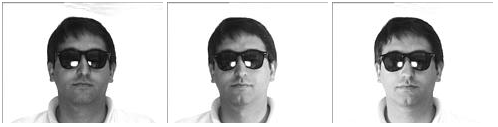
\includegraphics[scale=0.7]{figures/arface_example2} 
\newline
\caption{example of occlusion by sunglasses in the AR Face database}
\label{arface_example2}
\end{center} 
\end{figure}

\vspace{\baselineskip}
\begin{figure}[!h]
\begin{center}
\noindent 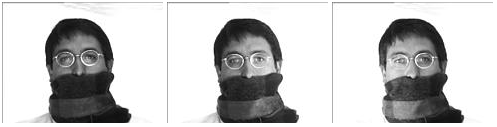
\includegraphics[scale=0.7]{figures/arface_example3} 
\newline
\caption{example of occlusion by scarf and glasses in the AR Face database}
\label{arface_example3}
\end{center} 
\end{figure} 

\noindent lignthing
\newline

\noindent angle
\newline

\phantomsection
\section{Requirements}

\vspace{\baselineskip}
\noindent bla bla bla
\newline




\stopcontents[parts]
